\chapter{Results}\label{Chap:Results}
In this chapter, the results from the FLEXPART and FLEXDUST model simulations are presented. 
The results from the model sensitivity experiments and validation are presented first in \Cref{sec:sensitvity_experiment} and \Cref{sec:model_eval} respectively. 
The rest of this Chapter will focus on interpreting the results from the 20-year simulation of springtime deposition to the \acrshort{clp}. 
In \Cref{sec:result_average} the climatology of the East Asian dust cycle is investigated.   
Before the inter-annual variations in dust  emissions, transport and deposition are examined in \Cref{sec:inter_annual_results} and how the covariability of springtime deposition is related to the large scale circulation. 
% For each location the mean dust transport path and main source regions are determined for both the clay and silt particle size bins. 

% Then in \Cref{sec:inter_annual_results} the inter annual variation in spring dust emissions, transport and deposition over the 20 year period are investigated. The composite analysis of the of the circulation during the preceeding winter in strong and weak deposition years show a strong positive MSLP anomalies over the arctic implying a negative \acrshort{ao}.   

\section{Model sensitivity to input data and parameters}\label{sec:sensitvity_experiment}
The sensitivity analysis aimed to quantify the impact of errors, variability, and uncertainties in the input data on the predicted model output. 
In \Cref{sec:sens_forcing} the impact of meteorological forcing on the simulated dust emissions and deposition is examined by comparing ERA5 and ERA-Interim forced simulations. 
Sand and clay fractions are important input variables in FLEXDUST (\Cref{sec:flexdust}), therefore the sensitivity of simulated dust emission to the choice of soil texture data set is considered in \Cref{sec:sens_soil}. 
In \Cref{sec:density_experiment} and \Cref{wet:dep_sensitivty} the impact particle density and below cloud scavenging on the estimated deposition investigated. 
\subsection{Forcing data}\label{sec:sens_forcing}

\begin{figure}[htpb]
    \centering
    \includegraphics[width=\textwidth]{texfiles/figs/emissions_ERA5_ERA-interim.pdf}
    \caption{Accumulated emission flux  (\si{\kg\per\square\metre}) simulated by FLEXDUST for the spring of 2015. (a) ERA5 0.3\degree resolution and (b) ERA-Interim 1\degree resolution. (c) The time series of daily accumulated emissions ERA-interim (red) and ERA-5 (black) }
    \label{fig:ERA5_ERA-interim_emissions}
\end{figure}
To better understand how possible errors and differences in the meteorological forcing impact the model results, FLEXPART and FLEXDUST simulations forced by ERA5 where compared to ERA-Interim forced simulations during the spring of 2015. Compared to ERA-interim, ERA5 features a more recent version of the IFS, higher spatial resolution 0.3\degree compared to 1\degree and increased number of vertical levels. 

\Cref{fig:ERA5_ERA-interim_emissions} shows the dust emission flux simulated by FLEXDUST with (a) ERA5 and (b) ERA-Interim. 
The impact of the coarser resolution of ERA-Interim is noticeable.  
Modelled dust emissions over the Taklamakan are particularly sensitive to the spatial resolution of the forcing. 
The coarse spatial resolution of ERA-Interim cannot resolve the complex topography of the surrounding Taklamakan desert. Moreover, mesoscale cold fronts typically produce dust storms in the Taklamakan desert, and these mesoscale fronts might be unresolved in ERA-interim due to its coarse resolution. 
Another feature missing in the ERA-Interim simulation is the boundary between Mongolia and the deserts northwest of the CLP. There are also major differences in the temporal evolution of simulated dust emissions (\Cref{fig:ERA5_ERA-interim_emissions}c) both in the magnitude and frequency.
In the ERA-Interim simulation, the most intense dust events show higher dust emissions compared to ERA5. However, for the weaker dust events, the opposite is true. This suggests that large dust storms, usually caused by synoptic scale frontal activity, are less sensitive to the resolution of the forcing compared to the weaker dust events.

\begin{figure}[htbp]
    \centering
    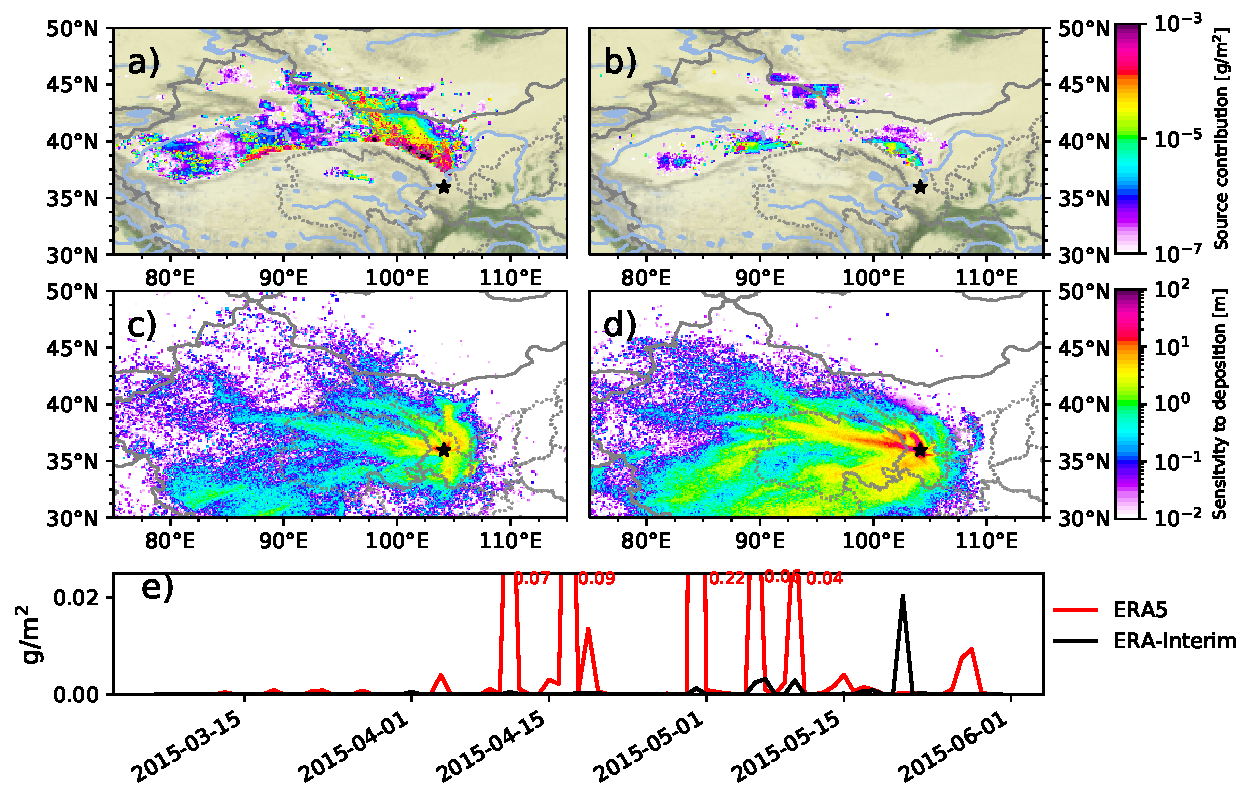
\includegraphics[width=\textwidth]{texfiles/figs/era5_era_interim_depo_tranpsort.pdf}
    \caption{Accumulated source contribution and emission sensitivity for ERA5 (a),(b) and ERA-interim (b),(d) for total deposition of "silt" during the spring of 2015. (e) time series of daily accumulated emission flux for ERA5 (red) and ERA-Interim (black).}
    \label{fig:era5_era_interim_source}
\end{figure}

Furthermore, the source contribution of total deposition (\Cref{fig:era5_era_interim_source}) is even more sensitive to input forcing. 
This might be partly because of ERA-Interim forced simulation having less emissions from weak and moderate dust events than the ERA5 forced simulation. 
This is also consistent with the largest deposition episode not coinciding with the strong emission events.
\subsection{Soil texture data}\label{sec:sens_soil}
The dust emission scheme used in FLEXDUST assume that the sandblasting efficiency (\Cref{eq:sand_blasing_eff}) increases exponentially with $f_{clay}$ for $f_{clay} \leq 0.2$. Consequently the simulated dust emission might be very sensitive to the soil texture data set used.
During the process of performing these sensitivity experiments, I discovered that the original soil texture dataset had a very small clay fraction over the Taklamakan (\Cref{fig:clay_sand_fraction_comparison}a). This resulted in FLEXDUST barely simulating any emissions from the Taklamakan desert.

\begin{figure}[hptb]
    \centering
    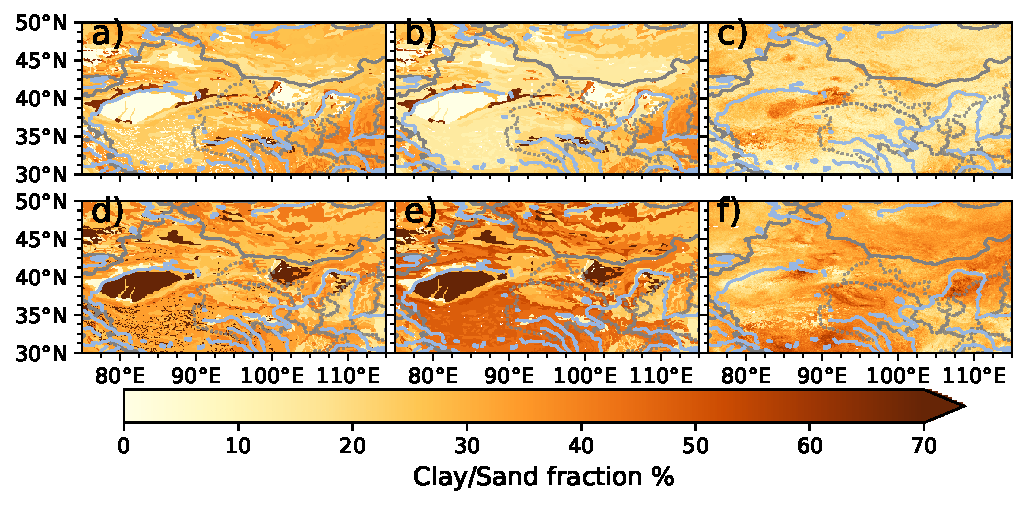
\includegraphics[width=\textwidth]{texfiles/figs/clay_sand_fraction.pdf}
    \caption{Clay and sand fraction maps from 3 different data sources: default clay (a), CLM clay (b), ISRIC clay (c), default sand (d), CLM sand (e) and ISRIC sand (f)}
    \label{fig:clay_sand_fraction_comparison}
\end{figure}

This bias was addressed by implementing new sand and clay maps in FLEXDUST based on the SoilGrids database developed by ISRIC.  The SoilGrids soil maps use state-of-the-art machine learning methods to map the spatial distribution of soil properties across the globe.
Providing a map of soil properties at 250 meter spatial resolution. 
As shown in \Cref{fig:clay_sand_fraction_comparison} ISRIC clay and sand fractions have a higher clay fraction over Taklamakan compared to the default soil maps. 
The accumulated modelled emissions for 2019 are shown in \Cref{fig:emissions_ISRIC_old_com}, (a) using the default soil maps and (b) with new ISRIC maps. 
The difference between the two is noticeable, with the new ISRIC maps, Taklamakan is now represented as a major dust source.

\begin{figure}[htpb]
    \centering
    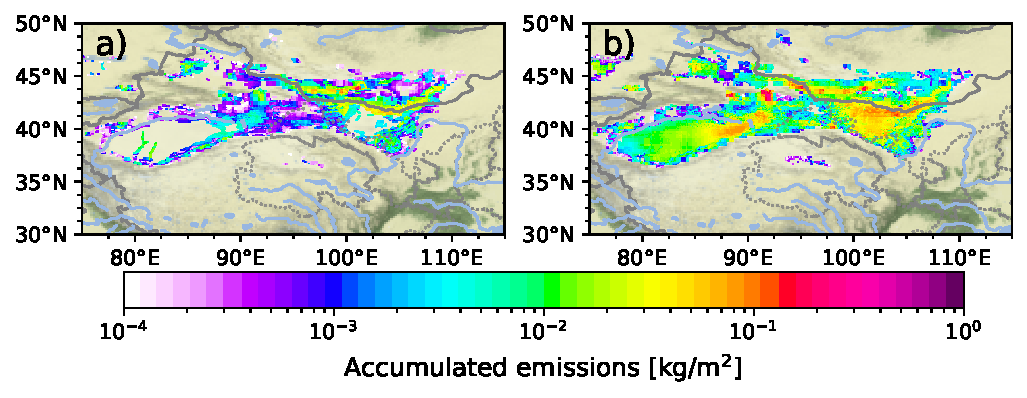
\includegraphics[width=\textwidth]{texfiles/figs/emssion_field_old_vs_isric_2019.pdf}
    \caption{Accumulated simulated dust emissions for 2019, default soil maps (a), and ISRIC soil maps (b).}
    \label{fig:emissions_ISRIC_old_com}
\end{figure}
\subsection{Particle density}\label{sec:density_experiment}
The density of a dust particle varies depending on its mineralogical composition. 
To assess how the density of the dust particle affects the long-range transport and the amount of deposited material,
FLEXPART simulations with varying particle density from \SI{2200}{\kg\per\cubic\cm} to \SI{2800}{\kg\per\cubic\cm}  were conducted from the SACOL site. 
In \Cref{fig:dry_dep_density} and \Cref{fig:wet_dep_density} the rate of dry and wet deposition are plotted for different densities and a least-squares fit is done to the data. 
The deposition rate increases approximately linearly with increasing particle density. 
The density has a bigger impact on the deposition rate of the coarse particles (\Cref{fig:dry_dep_density}b, \Cref{fig:wet_dep_density}), where the rate of deposition of the heaviest particle is almost twice that of the lightest particle. 
The fine particles only show about a 2\% difference between the lightest and heaviest particles in the dry deposition rate. 
The wet deposition is more sensitive to the particle density than the dry deposition for both the fine and coarse particles, possibly since the dust has to be lifted to high altitudes to be scavenged inside the clouds. 
\begin{figure}[hptb]
    \centering
    \includegraphics[width=\textwidth]{texfiles/figs/drydep_function_of_density.pdf}
    \caption{Dry deposition rate at the SACOL site as a function of dust particle density, (a) clay and (b) silt}
    \label{fig:dry_dep_density}
\end{figure}

\begin{figure}[hptb]
    \centering
    \includegraphics[width=\textwidth]{texfiles/figs/wetdep_function_of_density.pdf}
    \caption{The wet deposition rate at the SACOL site as a function of dust particle density, (a) clay and (b) silt}
    \label{fig:wet_dep_density}
\end{figure}

\subsection{Below cloud scavenging}\label{wet:dep_sensitivty}
To examine how much of wet deposition modelled wet deposition is due to below cloud scavenging. FLEXPART was run with and without the below cloud scavenging turned on. 
\Cref{fig:scav_sensitivty} shows the difference between having the below cloud scavenging scheme turned on and off. 
There is a higher contribution from the proximal regions with the below cloud scavenging turned on, which is expected since below cloud scavenging is the most efficient close to the source region.  
\begin{figure}[htbp]
    \centering
    \includegraphics[width=\textwidth]{texfiles/figs/no_scav_test.pdf}
    \caption{The difference in the source contribution to the wet deposition at BADOE. With below cloud scavenging turned on minus below cloud scavenging turned off.}
    \label{fig:scav_sensitivty}
\end{figure}

\section{Model evaluation against observation}\label{sec:model_eval}

\Cref{fig:model_eval_dry_deposition} shows the time series of observed and modelled monthly dry deposition fluxes from January 2009 until December 2010 for the four sites at the coast of Japan, as described in \Cref{sec:model_eval_discription}. 
Evident is FLEXPART ability to reproduce the spatial variation between the sites, with Fukuoka and Toyama experiencing the strongest deposition.
In both the observations and model, the deposition is strongest in spring and weakest in summer. 
The interannual variation between the two years is well captured by the model, with stronger deposition during 2010 compared to 2009 in both the observation and the model.
\begin{figure}[hptb]
    \centering
    \includegraphics[width=\textwidth]{texfiles/figs/monthly_accumulated_dry_depostion_japan.pdf}
    \caption{Dry deposition of dust simulated at 4 locations by the coast of Japan. The measurements of monthly deposition flux are described by \textcite{osada2014wet}}
    \label{fig:model_eval_dry_deposition}
\end{figure}
\Cref{fig:model_eval_wet_deposition} as in \Cref{fig:model_eval_dry_deposition} except for wet deposition.

For wet deposition, the agreement between the model and observation is worse.
Still, the spatial difference between the sites is retained and the difference in total emissions between the two years. 
However, when looking at the individual months,  the agreement between the model and observations is low. 
Especially odd is the extreme wet deposition in July of 2009 at the Fukuoka and Toyama site simulated by FLEXPART. 


\begin{figure}[hptb]
    \centering
    \includegraphics[width=\textwidth]{texfiles/figs/monthly_accumulated_wet_depostion_japan.pdf}
    \caption{Wet deposition of dust simulated at 4 locations off the coast of Japan. The measurements of monthly deposition flux are described by \textcite{osada2014wet}}
    \label{fig:model_eval_wet_deposition}
\end{figure}

\section{Climatology of the East Asian dust cycle}\label{sec:result_average}
To give some context to the investigation of the interannual variation of the East Asian dust cycle in \Cref{sec:inter_annual_results}. The multi-year average of dust emission, transport and deposition is examined first. 
\subsection{Emissions}
The dust cycle begins with dust emission.
The spatial distribution of the multiyear mean simulated dust emissions is shown in \Cref{fig:emission_map_flexdust}. 
The source regions are divided into five regions as shown in \Cref{fig:emission_map_flexdust}, namely; Taklamakan, Junggar Basin, Qaidam Basin, Mongolia and the northwest \acrshort{clp}. 
Of these five regions, the largest dust producers are the northwest \acrshort{clp}, Taklamakan and Mongolia \Cref{tab:emissions}. 
In total, FLEXDUST estimates approximately 11Mt/spring of dust emitted from the East Asian sources, which is less than the estimates by \textcite{xuan2004identification}. 
However, more importantly is whether FLEXDUST is able to capture the spatial distribution of the dust sources. 
FLEXDUST show a similar spatial distribution to \textcite{liu2018influence}, with the east to west source distribution showing increasing emissions between 110 \degree E - 95 \degree E, and with increasing emissions again at the entrance of the Tarim basin that decreases towards the western end of the basin (\Cref{fig:emission_map_flexdust}).    
% The estimated mean total spring emissions are 20.02 Mt/spring and are close to the estimates by \textcite{xuan2004identification} for PM30 of 27.6 Mt/year. 
% The regions with the highest spring emission are identified as the arid regions north west of the \acrshort{clp},  (mean emissions of $6.12\si{Mt}/ \mathrm{spring}$), Taklamakan desert (mean emissions of $4.33\si{Mt} / \mathrm{spring}$) and Mongolia (mean emissions of $2.91\si{Mt} / \mathrm{spring}$). Additional minor dust sources include the Junggar Basin in the north west of China and the Qaidam Baisin close to the Tibetan plateau.  


\begin{table}[htpb]
\caption{The mean emissions per spring for the three largest source regions}
\centering
\begin{tabular}{@{}
>{\columncolor[HTML]{FFFFFF}}l 
>{\columncolor[HTML]{FFFFFF}}l 
>{\columncolor[HTML]{FFFFFF}}l @{}}
\toprule
 &  Emissions (Mt) &  Percentage (\%)\\ \midrule
Taklamakan & 1.96 & 19 \\
North west \acrshort{clp} & 3.33  & 31 \\
Mongolia &  1.54  & 14 \\
Remaining regions &  3.99 & 36 \\
Total &  10.83 & 100 \\ \bottomrule
\end{tabular}
\label{tab:emissions}
\end{table}


\begin{figure}[hptb]
    \centering
    \includegraphics[width=\textwidth]{texfiles/figs/emission_map_1999_2019.pdf}
    \caption{Map of spring averaged dust emission flux simulated by FLEXDUST. The major source regions are indicated,  Junggar Basin \emph{(Red)},  Taklamakan (\emph{Blue}),  Qaidam Basin (\emph{Purple}), northwest CLP (\emph{Green}),  Mongolia \emph{(Orange)}}
    \label{fig:emission_map_flexdust}
\end{figure}

\subsection{Transport}
The averaged path the dust is transported along can tell a lot about the typical weather the dust encounters en route.    
Therefore, multi-year mean dust loading transport trajectories for all the receptor sites were calculated.
% The average dust loading trajectories are calculated based on the centroid trajectory of each particle release and in the averaging procedure, each centroid trajectory are given a weight based on their dust loading. 
\Cref{fig:dust_loading_trajecs}a and b shows the mean dry deposition dust loading trajectories for the clay and silt particles, respectively, with their accompanying vertical profiles shown in \Cref{fig:dust_loading_trajecs}c and d. Similarly wet deposition dust loading trajectories are shown in \Cref{fig:dust_loading_trajecs}e - h. 
The red points in \Cref{fig:dust_loading_trajecs} are spaced equally 12 hours apart and to indicate the velocity of dust transporting air masses. 
\begin{figure}[hptb]
    \centering
    \includegraphics[width=\textwidth]{texfiles/figs/average_dust_transport_trajectories.pdf}
    \caption{The weighted average of centroid dust loading trajectories for all the receptor locations during springtime from 1999-2019. (a) and (b) is the dry deposition dust loading trajectories for "clay" and "silt" respectively, (c) and (b) is their accompanying vertical path.  (e)-(f) as (a)-(b) just for wet deposition dust loading trajectories. The red points are spaced at 12 hours apart, indicating the speed of the dust transporting airmasses }
    \label{fig:dust_loading_trajecs}
\end{figure}

The dry deposited dust is transported along a similar northeasterly trajectory for both clay and silt particles. 
The exception is SACOL, where the coarse particles follow a more westerly trajectory. 
The air masses carrying the silt particles move faster compared to clay particles.  
The vertical profile of the averaged trajectories shows that the altitude of the dry deposited dust approximately decreases linearly with time. 
The height of the fine dust particles decreases more slowly with time compared to the coarse dust particles. 
This suggests that the transport of coarse dust from the remote source regions have to involve upper tropospheric transport. 
Compared to the fine dust particles, which are primarily transported through the lower troposphere regardless of the proximity of the source. 
This is also consistent with the coarse dust being transported more swiftly.  

Compared to the dry deposited dust, the wet deposited dust follow a more southerly trajectory.
The spread between the wet deposition trajectories is larger than the dry deposition trajectories, indicating that the source of the wet deposited dust is more site-dependent.
The vertical profile of the wet deposition show lifting starting approximately 12 hours before arriving at the receptor. 
Precipitation over the \acrshort{clp} during spring is usually caused by convection initiated by frontal activity. \Cref{fig:dust_loading_trajecs}g-h then shows the average time window between the wet deposition event and the start of the frontal lifting. Moreover this also gives an approximation of how long prior to deposition the dust would have to be entrained into the atmosphere, assuming that the dust have to be entrained before entering the frontal region.  
\subsection{Deposition}
\begin{figure}[htbp]
    \centering
    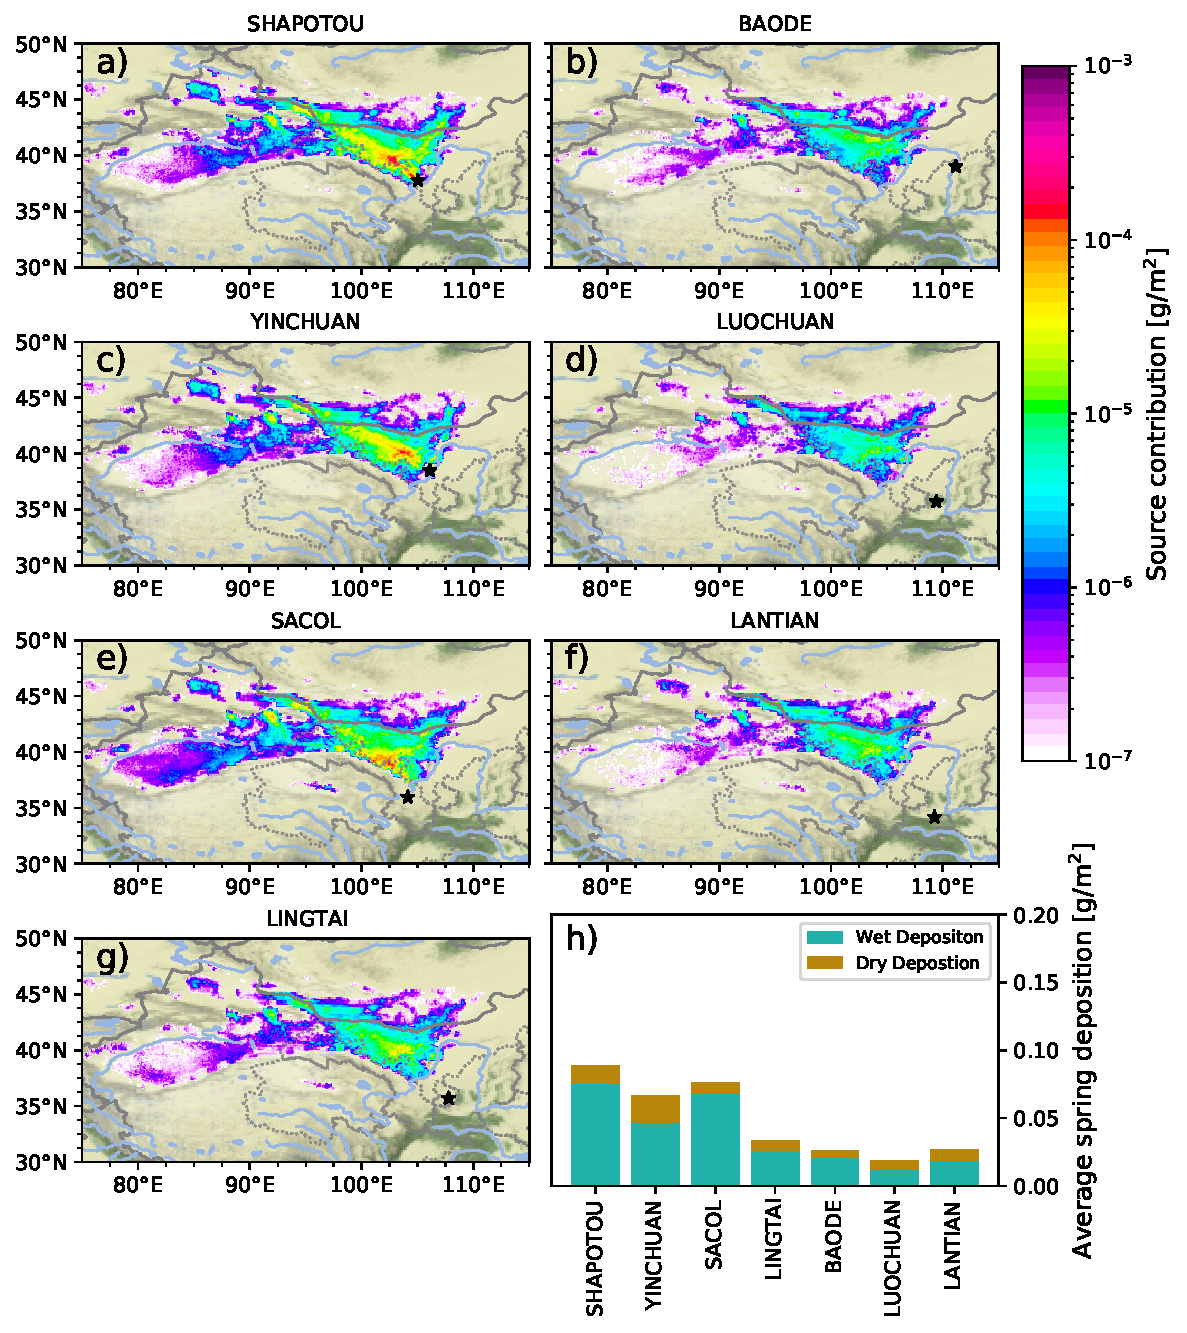
\includegraphics[width=\textwidth]{texfiles/figs/2micron_total_depositon_source_contribution.pdf}
    \caption{Yearly averaged spring source contribution "clay" dust size bin for the seven sites across the CLP (a-g). (h) shows the averaged spring deposition of each site for both wet- and dry deposition}
    \label{fig:source_contrib_2mmu}
\end{figure}

The advantage of using FLEXPART and FLEXDUST for modelling dust deposition is that it makes it possible to directly quantify how much each source region contributes to the deposition at the receptor.   
\Cref{fig:source_contrib_2mmu} and \Cref{fig:source_contrib_20mmu} shows the spring averaged source contribution for total deposition of the clay and silt particles respectively. 
The main source of the deposition at all  receptor locations is the  deserts northwest of the \acrshort{clp}. 
The western sites, Shapotou, Yinchuan, Sacol and Lingtai, have a stronger contribution from Taklamakan than the eastern sites. 
\Cref{fig:source_contrib_2mmu}h and \Cref{fig:source_contrib_20mmu}h shows that the primary mode of deposition for all the sites is wet deposition.
The wet deposition is even more dominating for the coarse particles. 
For coarse particles the areas with the largest contribution is located further away from the receptor compared to the fine particles as expected based on hypothesis that the coarse dust is particles mainly transported by faster moving air in the upper troposphere.
    
 \begin{figure}[htbp]
    \centering
    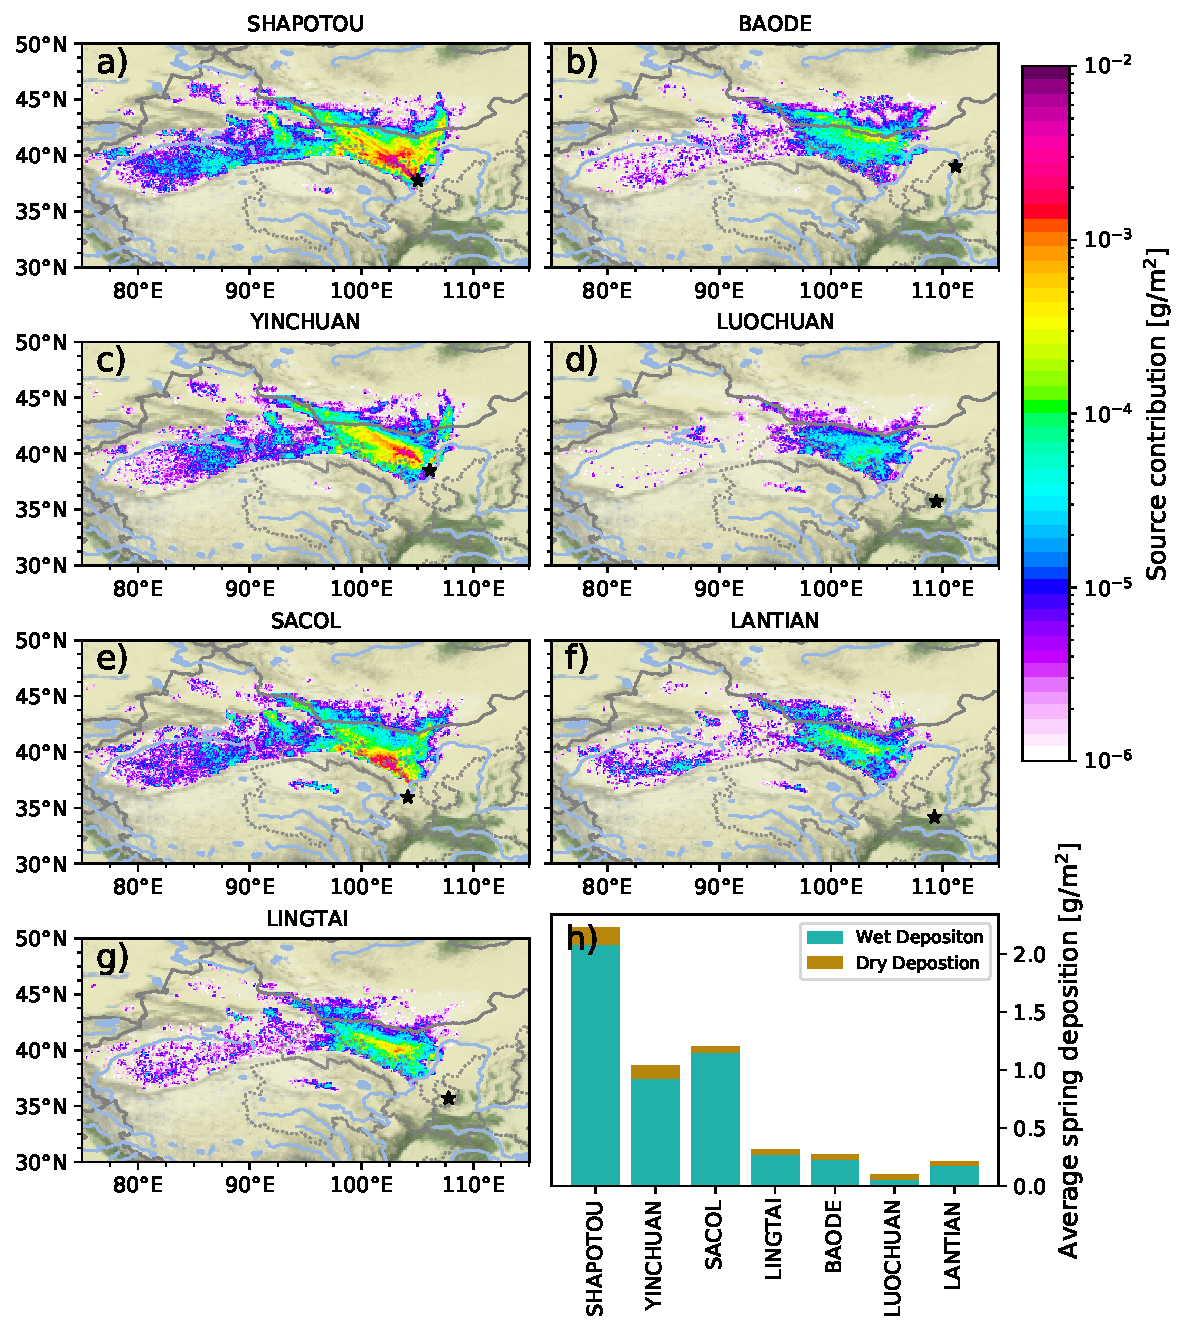
\includegraphics[width=\textwidth]{texfiles/figs/20micron_total_depositon_source_contribution.pdf}
    \caption{Yearly averaged March-May source contribution "silt" size bin for the seven sites across the \acrshort{clp} (a-g). Panel h) shows the averaged spring deposition of each site for both wet- and dry deposition}.
    \label{fig:source_contrib_20mmu}
\end{figure}

\section{Interannual variability of the East Asian dust cycle}\label{sec:inter_annual_results}

\subsection{Emissions}
The time series of springtime emissions for the 3 main source regions are shown in \Cref{fig:emission_timeseries}. Over this 20 year period, there is no evident long-term trend in the springtime dust emissions. 
The three years with the strongest overall dust emissions are identified as 2001, 2010 and 2018. For 2001 and 2010, the northwest \acrshort{clp} region stand for the main increase in emissions, whereas for 2018, Taklamakan and the smaller source regions are mainly responsible for the increased emission.
Years with strong emissions from the northwest CLP generally coincide with enhanced emissions from Mongolia but not always with enhanced emissions from Taklamakan, e.g. 2013.   

\begin{figure}[htbp]
    \centering
    \includegraphics[width=\textwidth]{texfiles/figs/emission_timeseries_1999_2019.pdf}
    \caption{Time series of total springtime dust emissions from 1999-2019. The total emission is partitioned into the contribution from the Taklamakan (Blue), North West CLP (Green) and Mongolia (Orange) }
    \label{fig:emission_timeseries}
\end{figure}

\acrfull{eof} analysis based on yearly de-trended spring emissions was done to identify spatiotemporal characteristics in dust emissions from the East Asian deserts.
The significance of each \acrshort{eof} was evaluated based on the rule of thumb outlined by \textcite{north1982sampling}. 
Stating that if the neighbouring eigenvalue lay within the typical error of the respective eigenvalue $\lambda$, the two EOFs might be mixed in their signal, thus not representing true patterns. Following this rule, 
\Cref{fig:eof_test} shows that the first and second \acrshort{eof} meets this criterion.  

\begin{figure}[htbp]
    \centering
    \includegraphics[width=\textwidth]{texfiles/figs/Emissions_EOF.pdf}
    \caption{The spatial pattern of the leading EOF (a) and second EOF (b). (c) the time series of the normalized principal component of the first (purple) and second (blue) EOFs.}
    \label{fig:emissions_eof}
\end{figure}
\Cref{fig:emissions_eof}a and b shows the spatial pattern of EOF1 and EOF2. EOF1 and EOF2 account for 54 \% and 12 \% of the total variance in annual springtime emissions. 
The leading EOF represents increased emissions across all the source regions. 
As expected, the years with a large positive principal component (PC) correspond to strong emission years (\Cref{fig:emissions_eof}c). 
Interestingly the second EOF shows a dipole pattern between emissions in Mongolia and Taklamakan. 
The signal of the second EOF is also visible from the time series where the positive EOF2 years correspond to a disproportional increase in emissions from Taklamakan compared to emissions from Mongolia and vice versa.       

Composite analysis of the preceding winter circulation for strong positive minus strong negative \acrshort{eof} years was done to understand better the kind of circulation anomalies that produces the spatial pattern identified by the \acrshort{eof} analysis. 
In positive EOF1 years, the composite anomalies indicate a negative \acrshort{ao} mode, with positive \acrshort{mslp} anomalies over the arctic region.
The composite anomalies for the second \acrshort{eof} show a weakened Aleutian low and Siberian high suggesting weak \acrshort{eawm} circulation.
In other words, the EOF analysis suggests increased emissions from Taklamakan during weak \acrshort{eawm} years. The weakend \acrshort{eawm} produces a weaker northwesterly winds, which could favour cold air intrusions into the Tarim basin.        
\begin{figure}[htpb]
    \centering
    \includegraphics[width=\textwidth]{texfiles/figs/EOF_emissions_composite.pdf}
    \caption{DJF composite anomalies of MSLP and 850hPa winds the strong positive minus strong negative  EOF1 (a) and EOF2 (b) years}
    \label{fig:eof_composite_DJF}
\end{figure}
The \acrshort{mam} composite (\Cref{fig:eof_composite_MAM}) shows how the circulation anomalies evolve into spring. 
The \acrshort{eof}2 spring composite of indicates a transition to a positive \acrshort{ao} like circulation pattern with negative \acrshort{mslp} anomalies over the arctic. 
Moreover, there is now a negative pressure anomaly over Taklamakan causing easterly wind anomalies in the Tarim Basin.
The southwesterly wind anomalies could explain the reduction in emissions over Mongolia. 
\begin{figure}[htpb]
    \centering
    \includegraphics[width=\textwidth]{texfiles/figs/EOF_emissions_composite_MAM.pdf}
    \caption{\acrshort{mam} composite anomalies of MSLP and 850hPa winds the strong positive minus strong negative  EOF1 (a) and EOF2 (b) years}
    \label{fig:eof_composite_MAM}
\end{figure}

\subsection{Dust transport}
\begin{figure}[htbp]
    \centering
    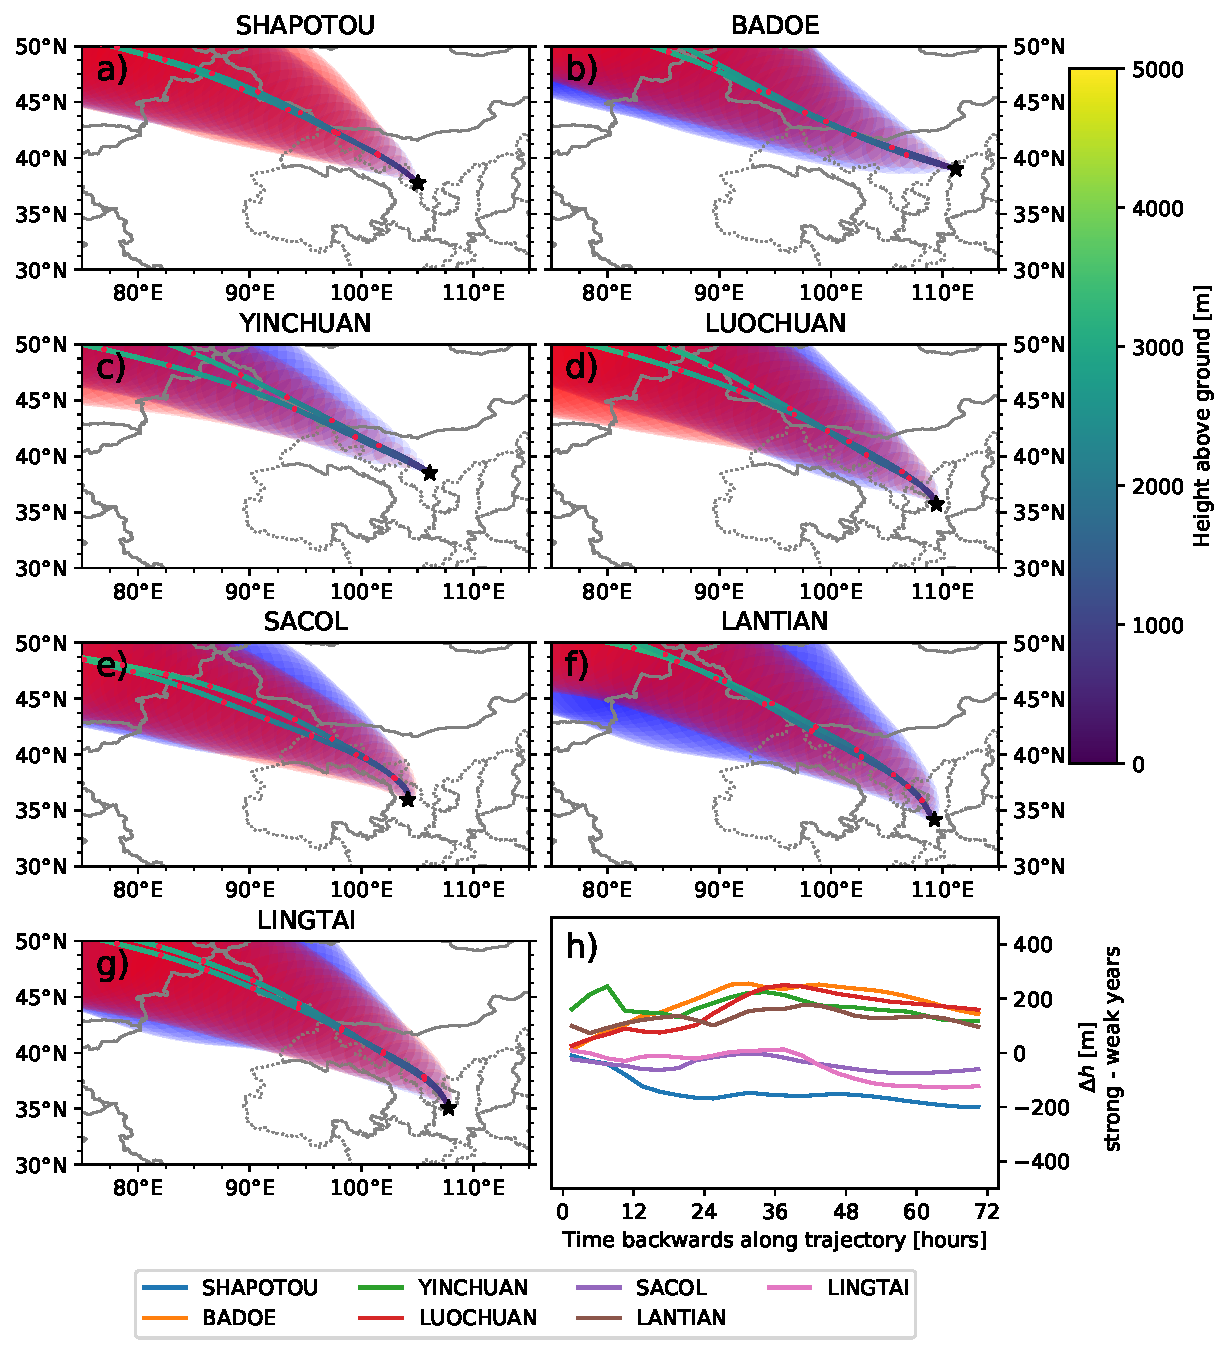
\includegraphics[width=\textwidth]{texfiles/figs/2_micron_drydep_weak_strong_trajecs.pdf}
    \caption{The weighted average of dry deposited clay dust loading trajectories for strong (red diamonds) and weak deposition (blue circles) years for every location. The standard deviation of the trajectories during the weak deposition and strong deposition years are represented by the blue and red shading respectively.  (h) show the difference in height of the dust transporting air masses during strong and weak deposition years. }
    \label{fig:strong_weak_drydepo_year_2mmu_trajecs}
\end{figure}

Examining the differences in transport between strong and weak deposition years can provide insight on how the dust transport to the \acrshort{clp} is different in periods with high and low \acrshort{mar}. 
% The differences in transport between the weak and strong deposition years for all the receptor locations were examined by taking the weighted mean of the centroid trajectories during weak and strong wet and dry deposition years for both the fine and coarse particle size bins. 
\Cref{fig:strong_weak_drydepo_year_2mmu_trajecs} and \Cref{fig:strong_weak_drydepo_year_20mmu_trajecs} shows the dry deposition dust loading trajectories for the clay and silt particle size bin in weak and strong deposition years. 
The standard deviation during strong and weak years is shaded red and blue, respectively; the purple region is where the two overlap. 
During strong deposition years, the spread of the trajectories is generally narrower and more condensed to a northwesterly direction.
Suggesting a more organised dust transport path and source areas in strong deposition periods.   
Moreover, the dust during strong dry deposition years is transported more swiftly than in weak deposition years. 
Caused by the dust being transported through higher altitudes during the strong deposition years \Cref{fig:strong_weak_drydepo_year_20mmu_trajecs}h.
% The exception is the transport of fine dust to Shapotau and SACOL, located in close proximity to the sources regions. 
% This suggest that dry deposition of fine dust at these two locations might be most favourable during moderate dust events.


\begin{figure}[htbp]
    \centering
    \includegraphics[width=\textwidth]{texfiles/figs/20_micron_drydep_weak_strong_trajecs.pdf}
    \caption{The weighted average of dry deposited silt dust loading trajectories for strong (red diamonds) and weak deposition (blue circles) years for every location. The standard deviation of the trajectories during the weak deposition and strong deposition years is represented by blue and red shading. (h) show the difference in height of the dust transporting air masses during strong and weak deposition years. }
    \label{fig:strong_weak_drydepo_year_20mmu_trajecs}
\end{figure}


\begin{figure}[htbp]
    \centering
    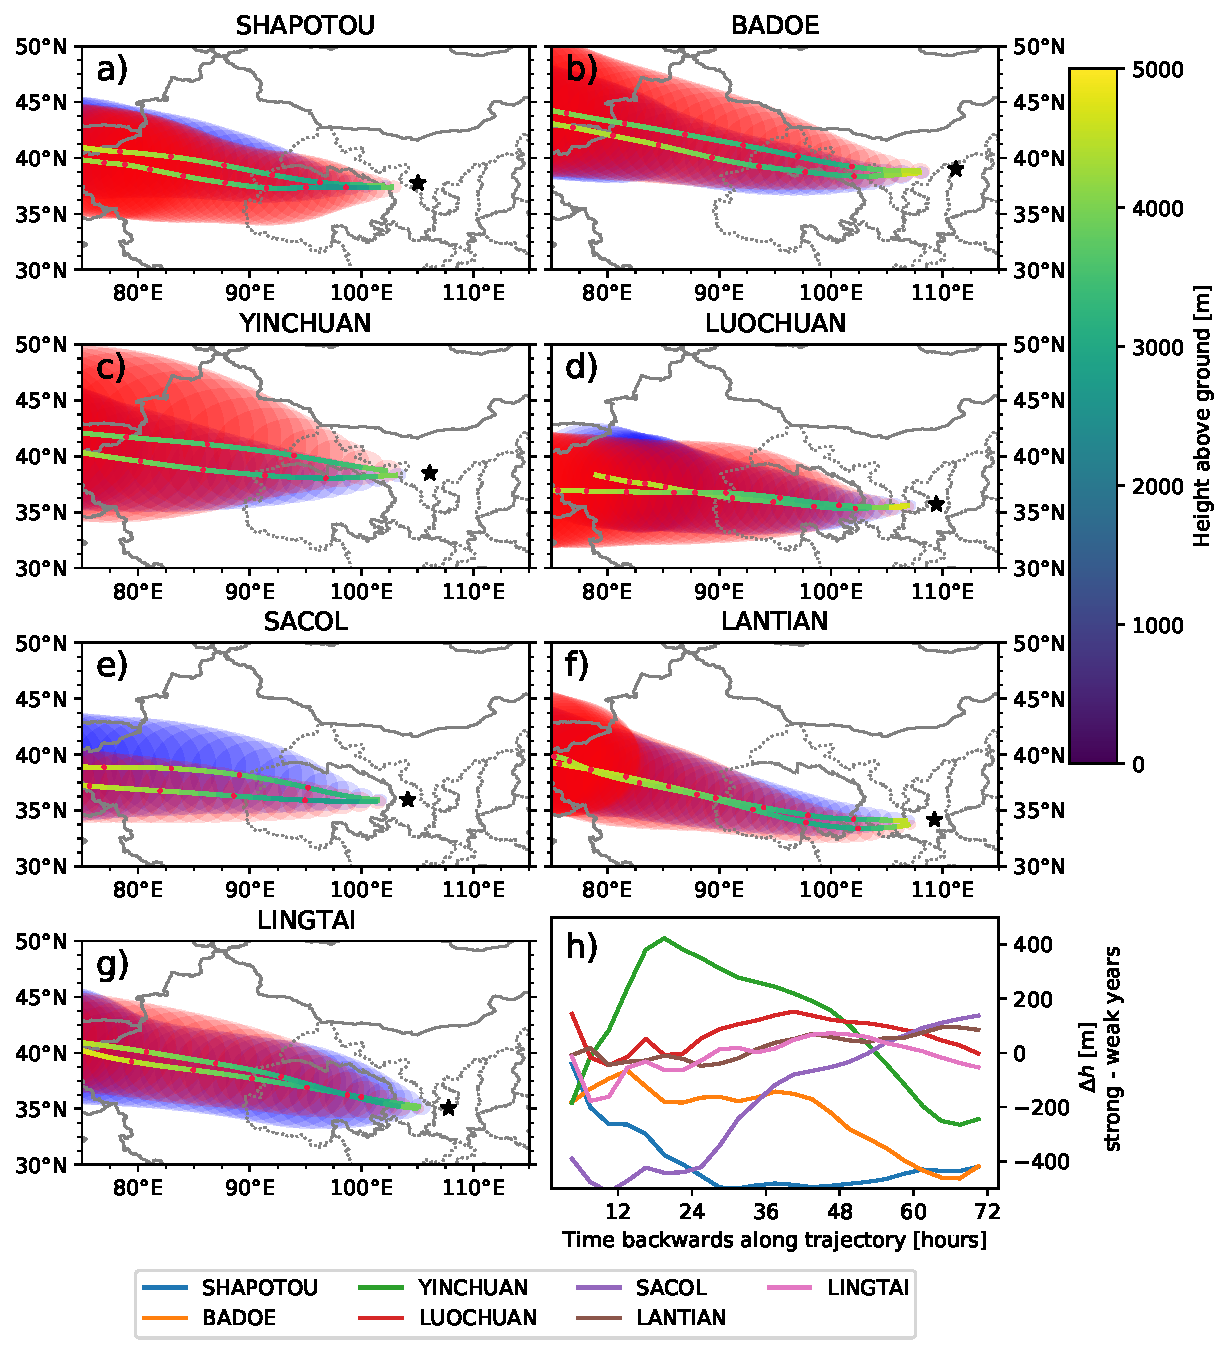
\includegraphics[width=\textwidth]{texfiles/figs/2_micron_wetdep_weak_strong_trajecs.pdf}
    \caption{The weighted average of wet deposited clay dust loading trajectories for strong (red diamonds) and weak deposition (blue circles) years for every location. The standard deviation of the trajectories during the weak deposition and strong deposition years is represented by blue and red shading.  (h) show the difference in height of the dust transporting air masses during strong and weak deposition years. }
    \label{fig:strong_weak_wetdepo_year_2mmu_trajecs}
\end{figure}
The prerequisite conditions involved in wet deposition occur more randomly, and thus as not strongly influenced by changes in the mean winds. 
Therefore it is hard to make a general statement about the transport of wet deposited dust, besides that years with strong deposition the dust is transported by faster moving air masses compared to weak deposition years. 
As with the multiyear averaged wet deposition trajectories, the differences in dust transport trajectories between weak and strong wet deposition years are mostly site specific. 
% SACOL, Lingtai, Lantian

\begin{figure}[htbp]
    \centering
    \includegraphics[width=\textwidth]{texfiles/figs/20_micron_wetdep_weak_strong_trajecs.pdf}
    \caption{The weighted average of wet deposited silt dust loading trajectories for (red diamonds) and weak deposition (blue circles) years for every location. The standard deviation of the trajectories during the weak deposition and strong deposition years is represented by blue and red shading.  (h) show the difference in height of the dust transporting air masses during strong and weak deposition years. }
    \label{fig:strong_weak_wetdepo_year_20mmu_trajecs}
\end{figure}

\subsection{Source contribution}

From the mineralogy of the loess deposits, it is possible to differentiate the provenance of deposited dust in periods of high and weak \acrshort{mar}. Conversely similarly the question can be examined with FLEXPART by comparing the source contribution during weak and strong deposition years.  
\Cref{fig:source_contrib2mmu_anomalies} shows the normalised source contribution for the "clay" particle size bin. The model result suggests that strong deposition years have a more concentrated source contribution. 
The exception is SACOL (\Cref{fig:source_contrib2mmu_anomalies}e) which during strong deposition years has increased contribution from the entire region northwest of the \acrshort{clp}. 
During strong deposition years, the more concentrated source contribution suggests that the strong deposition years are set apart from the weak deposition years by having a large contribution from rare strong dust events. 
By comparison, the weak deposition years the source regions are more randomly distributed. \Cref{fig:source_contrib20mmu_anomalies} is as the previous figure just for the "silt" particle size bin and tells much of the same message. 
However, Lantian which has reduced deposition from Taklamakan during strong deposition years for the fine particle size bin show increased contribution from Taklamakan during strong deposition years.     
\begin{figure}[hptb]
    \centering
    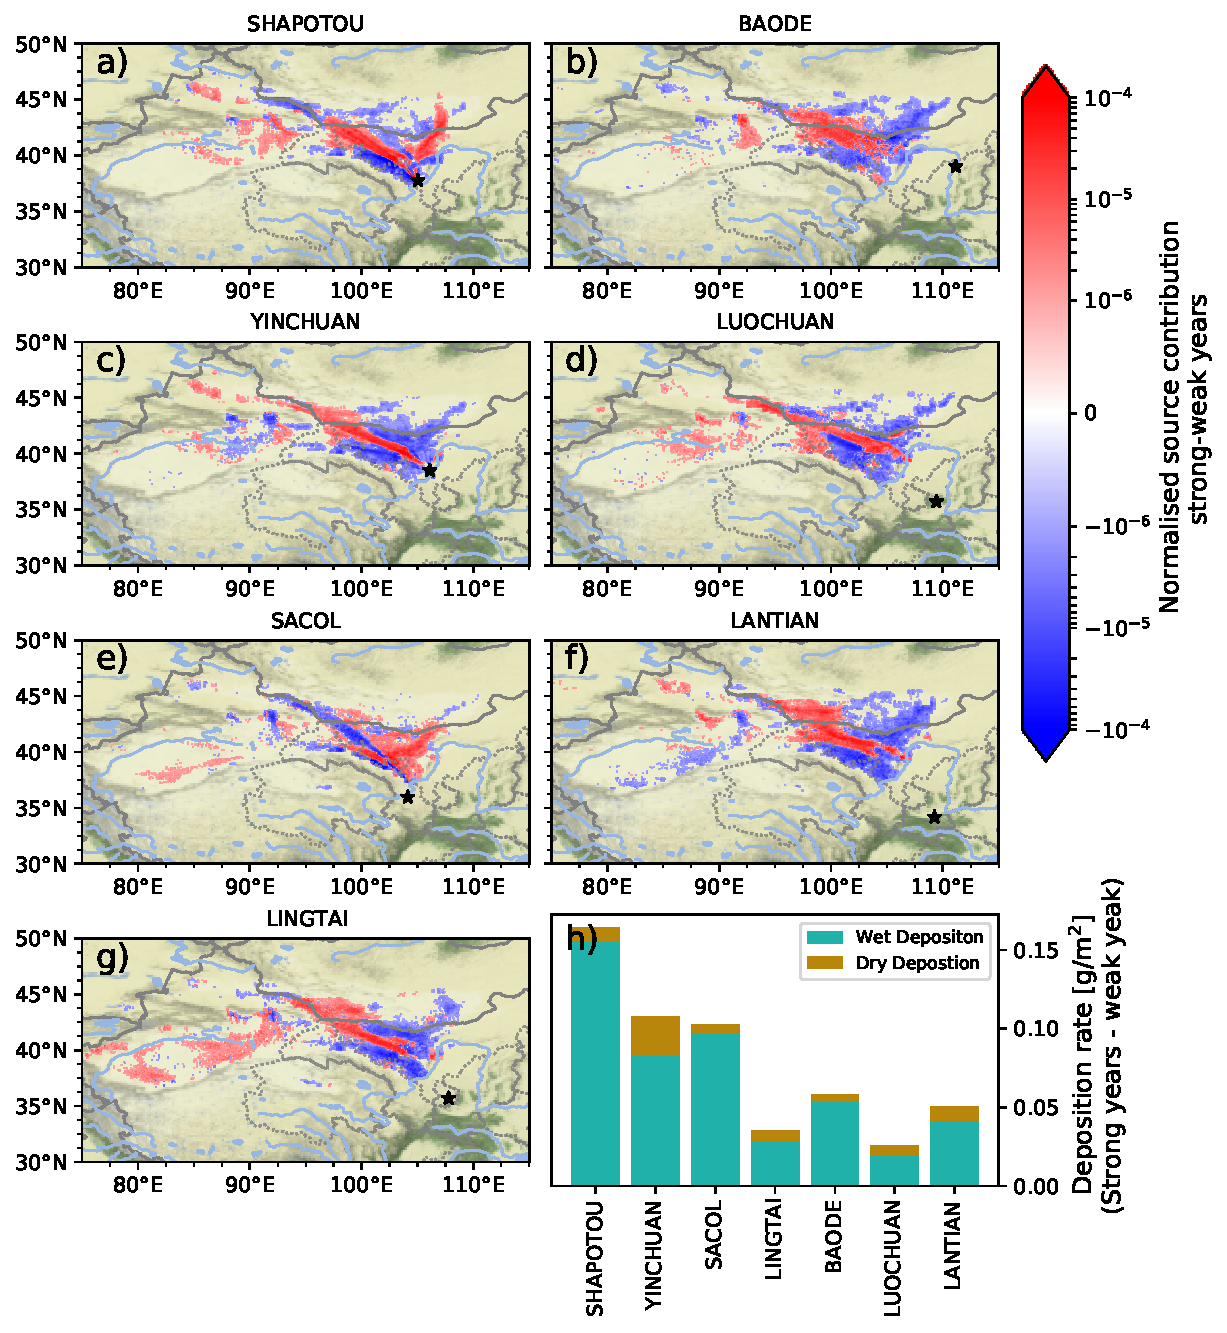
\includegraphics[width=\textwidth]{texfiles/figs/composite_source_contrib_2micron_tot_dep.pdf}
    \caption{Normalised source contribution composite anomalies of "clay" particle size bin for all locations, strong - weak deposition years.}
    \label{fig:source_contrib2mmu_anomalies}
\end{figure}

\begin{figure}[hptb]
    \centering
    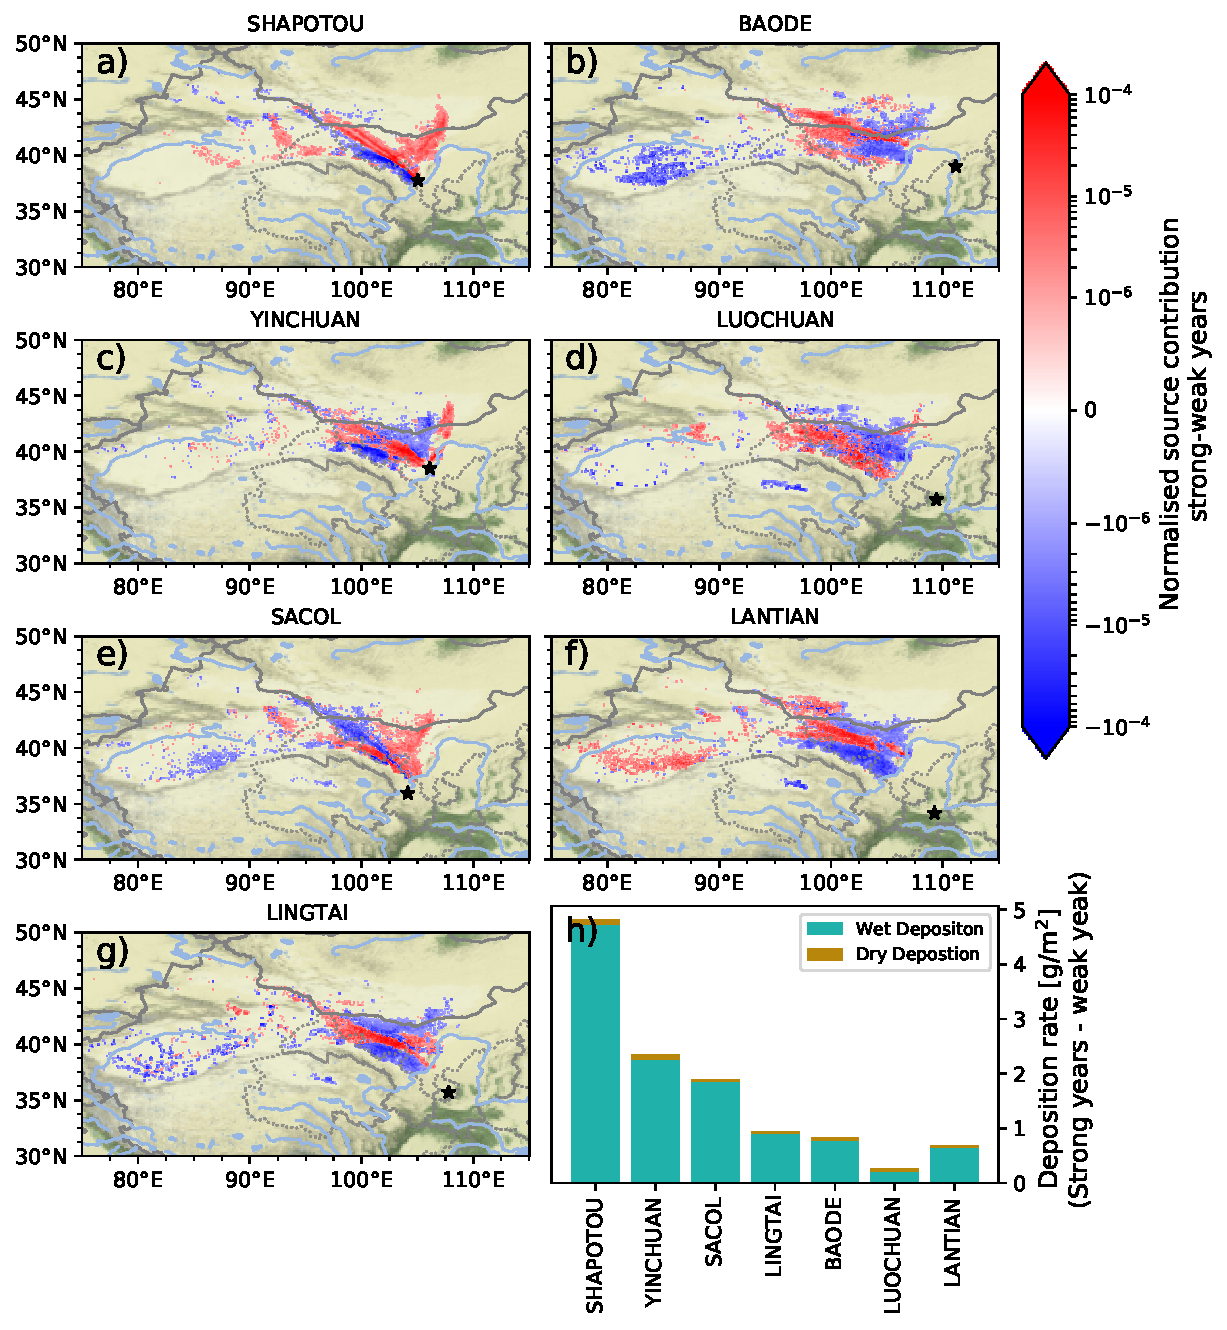
\includegraphics[width=\textwidth]{texfiles/figs/composite_source_contrib_20micron_tot_dep.pdf}
    \caption{Normalised source contribution composite anomalies of "silt" particle size bin for all locations, strong - weak deposition years.}
    \label{fig:source_contrib20mmu_anomalies}
\end{figure}

\subsection{Covariations of spring deposition and large-scale circulation patterns}
To analyse the influence of regional and large scale circulation changes on the \acrshort{mar} over the \acrshort{clp}. 
Correlation analysis between deposition at each site and several regional and large-scale climate indices. \todo{make table}.
The circulation indices are calculated based seasonally averaged ERA5 reanalysis. 
The full analysis is shown in \Cref{fig:correlations} and the significant correlations are displayed. 
The winter \acrshort{ao} and \acrshort{nao} show the strongest correlation with dust deposition of all the indices considered in this analysis. 
Contradictory to previous research, there is only a very weak correlation between the \acrshort{eawm} and deposition. 

\begin{figure}[htpb]
    \centering
    \includegraphics[width=\textwidth]{texfiles/figs/correlations.pdf}
    \caption{Interannual correlations between deposition and each site and local and large-scale climate indices. The significant correlations are indicated}
    \label{fig:correlations}
\end{figure}

To examine the covariability between the emission strength in the different source regions and deposition at the receptor locations correlation analysis between deposition and emissions were also included. 
The dry deposition is strongly correlated with emissions in Mongolia and the northwest \acrshort{clp} for almost all sites. However, only Lantian and SACOL show a significant correlation between emissions from Taklamakan and dry deposition. 
Moreover, wet deposition is generally not significantly correlated and emissions. 
The exception being Lantian which shows a significant positive correlation between emissions from Mongolia and northwestern sources. For the same reason wet deposition at Lantian also have a high correlation with dry deposition at the other sites.  

% This exemplifies the randomness of the occurrence of wet deposition events. 

% The correlations between deposition among the sites show that wet deposition at Lantian correlates well with dry deposition at almost all the other sites. 

\subsection{Circulation composites}

To better understand the circulation differences between strong and weak deposition years, composite differences anomalies were calculated by subtracting the circulation during strong minus weak deposition years. 
The circulation anomalies of \acrshort{djf} 850hPa winds and \acrshort{mslp} are shown in \Cref{fig:DJF_850_fine_composite} and \Cref{fig:DJF_850_coarse_composite} for the fine and coarse particles respectively.
Comparing the composite anomalies to the composite anomalies of strong \acrshort{ao} (\Cref{fig:mo_ao_composite}a) and \acrshort{eawm} (\Cref{fig:mo_ao_composite}b) the deposition composites are generally consistent with negative \acrshort{ao} circulation anomalies.
The exception being Badoe which seems to be more influenced by the pressure changes over the ocean. 




\begin{figure}[hp]
    \centering
    \includegraphics[width=\columnwidth]{texfiles/figs/mslp_850hPa_2micron_DJF.pdf}
    \caption{Composite difference anomalies of mean sea level pressure and 850hPa strong minus weak deposition years of the "clay" size bin in winter (DJF) for all the locations (a-g). (h) indicates which years are strong and which years are weak.}
    \label{fig:DJF_850_fine_composite}
\end{figure}

\begin{figure}[hp]
    \centering
    \includegraphics[width=\textwidth]{texfiles/figs/mslp_850hPa_20micron_DJF.pdf}
    \caption{Composite difference anomalies of mean sea level pressure and 850hPa strong minus weak deposition years of the "silt" size bin in winter (DJF) for all the locations (a-g).  (h) indicates which years are strong and which years are weak.}
    \label{fig:DJF_850_coarse_composite}
\end{figure}

\begin{figure}[htbp]
    \centering
    \includegraphics[width=\textwidth]{texfiles/figs/mslp_850hPa_2micron_MAM.pdf}
    \caption{Composite difference anomalies of mean sea level pressure and 850hPa strong minus weak deposition years of the "clay" size bin in spring (MAM) for all the locations (a-g).  (h) indicates which years are strong and which years are weak.}
    \label{fig:MAM_850_fine_composite}
\end{figure}

\begin{figure}[htbp]
    \centering
    \includegraphics[width=\textwidth]{texfiles/figs/mslp_850hPa_20micron_MAM.pdf}
    \caption{Composite difference anomalies of mean sea level pressure and 850hPa strong minus weak deposition years of the "silt" size bin in spring (MAM) for all the locations (a-g).  (h) indicates which years are strong and which years are weak.}
    \label{fig:MAM_850_coarse_composite}
\end{figure}


\begin{figure}[hptb]
    \centering
    \includegraphics[width=\columnwidth]{texfiles/figs/geopot_ws_500hPa_2micron_DJF.pdf}
    \caption{Winter (DJF) composite difference anomalies of 500hPa geopotential height (contours) and 500hPa wind speed (shading) strong minus weak deposition years of clay in winter (DJF) for all the locations a-g  (h) indicates which years are strong and which years are weak.}
    \label{fig:DJF_500hPa_fine_composite}
\end{figure}

\begin{figure}[hptb]
    \centering
    \includegraphics[width=\columnwidth]{texfiles/figs/geopot_ws_500hPa_20micron_DJF.pdf}
    \caption{Winter (DJF) composite difference anomalies of 500hPa geopotential height (contours) and 500hPa wind speed (shading) strong minus weak deposition years of silt for all the locations a-g  (h) indicates which years are strong and which years are weak.}
    \label{fig:DJF_500hPa_coarse_composite}
\end{figure}

\begin{figure}[hptb]
    \centering
    \includegraphics[width=\columnwidth]{texfiles/figs/geopot_ws_500hPa_2micron_MAM.pdf}
    \caption{Spring (MAM) composite difference anomalies of 500hPa geopotential height (contours) and 500hPa wind speed (shading) strong minus weak deposition years of clay for all the locations a-g  (h) indicates which years are strong and which years are weak.}
    \label{fig:MAM_500hPa_fine_composite}
\end{figure}

\begin{figure}[hptb]
    \centering
    \includegraphics[width=\columnwidth]{texfiles/figs/geopot_ws_500hPa_20micron_MAM.pdf}
    \caption{Spring (MAM) composite difference anomalies of 500hPa geopotential height (contours) and 500hPa wind speed (shading) strong minus weak deposition years of silt for all the locations a-g  (h) indicates which years are strong and which years are weak.}
    \label{fig:MAM_500hPa_coarse_composite}
\end{figure}
